% \documentclass[12pt,openright,oneside,a4paper,brazil]{abntex2}
% \usepackage[utf8]{inputenc}
% \counterwithout{section}{section}
% \counterwithout{figure}{chapter}
% \counterwithout{table}{chapter}
% \setlength{\parindent}{1.3cm}
% \usepackage{indentfirst}
% \setlength{\parskip}{0.2cm}
% \usepackage[bottom=2cm,top=3cm,left=3cm,right=2cm]{geometry}
% \usepackage{graphicx}
% \graphicspath{{figuras/}}
% \usepackage{placeins}
% \usepackage{url}
% \makeatletter
% \setlength{\@fptop}{0pt}
% \makeatother
% %opening
% \title{}
% \author{}
% 
% \begin{document}
% 
% 
% \textual
\begin{center}
 {\large Plano de gerenciamento de projeto}\\[0.2cm]
 {Planta de abastecimento de água potável a partir da umidade do ar}\\
 \end{center}
 
 \section*{Histórico de Alterações}
\begin{table}[h]
\centering
\begin{tabular}{|c|c|p{6cm}|p{5cm}|}

Data & Versão & Descrição & Responsável\\
\hline                               
24/04/2015 & 0.0 & Criação do Plano de Gerenciamento de projeto & Rafael Abreu de Carvalho\\
\hline

\end{tabular}
\end{table}

\section*{Objetivo}
  O objetivo desse plano é estabelecer um processo de gerenciamento para todo o projeto.
  
\section*{Visão Geral}
\begin{enumerate}
  
  \item Nome do projeto\\
  Plano de abastecimento de água potável a partir da umidade do ar.
  
  \item Descrição do projeto\\
  O projeto visa desenvolver uma planta de abastecimento de água potável, por meio de um sistema de captação a partir da umidade do ar na cidade de Acari-RN (município da Microrregião do Seridó Oriental, na região do Seridó), no bairro Vereador Tarcísio Bezerra Galvão. O bairro possui uma população de aproximadamente 900 habitantes e sofre constantemente com a falta de água. \\
  Seu foco gira em torno de uma solução tecnológica  capaz de retirar a água do ar  por processos químicos e físicos e tornar essa água potável e própria para o consumo humano de forma renovável e menos danosa possível. Para isso aplicamos conhecimentos das demais áreas da engenharia atuando no desenvolvimento e conceituação do projeto. Nossa estimativa e de que possamos produzir aproximadamente 3 mil litros de água por dia. Essa quantidade e suficiente para atender toda a população do município. \\
  O projeto conta com grupos que trabalham em áreas diferentes mas interligadas e com um único propósito. Cada etapa e gerida e coordenada por representantes de forma a garantir um resultado satisfatório com qualidade e que supra a necessidade da população da região.

  \item Objetivo do Projeto\\
  O projeto tem por objetivo a implementação de um sistema capaz de a partir da  umidade do ar fornecer água potável, de modo a suprir a demanda do bairro Vereador Tarcísio Bezerra Galvão situado em Acarí, RN, o  uso da água especialmente como elemento de desenvolvimento econômico, será de grande valia para os moradores locais.

  Contudo, para a aplicação prática da produção de água a partir da umidade do ar, é bastante verificar que, com uma umidade relativa de 60\%, que é a média mundial, um metro cúbico de ar carregará cerca de 18 gramas de água (considerando uma temperatura ambiente de $30\,^{\circ}\mathrm{C}$). 

  \item Justificativa do Projeto\\
  \begin{enumerate}[label=\Alph*]
  \item Por que deve-se pensar em projetos como esse?\\
  Atualmente, cerca de 40 \% da população mundial sofre com consequências da falta de água, além da sede faltam recursos hídricos, o que gera graves implicações na economia e política. De acordo com o geólogo Sjiklomanov, do Instituto Hidrológico Estadual de São Petesburgo, Rússia, em 2000 foi previsto que: “Os países em desenvolvimento vão aumentar seu uso de água em até 200\% em 25 anos”. Em 2014 no Brasil, foi evidenciado consequências desse aumento no consumo de água juntamente com fatores climático, resultando na falta de água em cidades de Pernambuco, Minas Gerais e São Paulo.
  Essa situação de falta de água não é nova, a ONU em 2003 já previa os futuros transtornos que seriam causados pela crise de água. O World Water Development Report, se destaca sobre o tema porque é um documento da ONU que também traz estudos mostrando como esse problema já afeta e mata milhares de pessoas. Este estudo prevê que 2,7 bilhões de seres humanos – 45\% da população mundial – vão ficar sem água no ano 2025.
  Diante dessa situação e de previsões sobre a falta de água tão breves, devem-se tomar medidas para minimizar a situação e planejar soluções para a produção de água potável buscando outras fontes, como o ar, por exemplo. Por isso, esse projeto visa através da umidade do ar, retirar água potável e planeja um estudo de abastecimento na cidade de Acari, RN.

  \item Por que  Acari foi a cidade escolhida?\\
  Na situação de crise hídrica vivida pelo país atualmente, observa-se grandes centros urbanos sofrendo com a falta de água para consumo humano (o que antes era praticamente exclusivo para a região do semiárido nordestino). Além disso, observa-se que a seca na região nordeste vem se agravando muito nos últimos anos, especificamente na região do Seridó, que fica no semiárido do RN.
  Dessa forma, soluções alternativas para o abastecimento de água potável a fim de atender o consumo humano fazem-se necessárias. Sendo assim, a região para a qual o sistema será projetado será o município de Acari – RN, pois é uma região onde há muita demanda (11303 habitantes) e tem sofrido muito com a escassez de água. A escolha dessa região baseia-se principalmente na questão social, uma vez que o projeto visa atender o consumo humano de pessoas que não tem acesso à água potável.
  Além de ser uma região que apresenta necessidade de um planejamento para a amenização ou suprimento da escassez de água, é também, uma região muito quente com temperatura média anual de 33Cº, pois está localizada no polígono das Secas (local de maior concentração de seca no país). Consequentemente, o volume de água do Açude de Gargalheiras, açude este que abastece a cidade, decai consideravelmente em épocas de seca, fazendo com que haja escassez de água na cidade. A possibilidade de retirar água potável do subterrâneo, é inviável pois a água é muito salobra. Apesar de clima quente e semi-árido a umidade do ar nessa região  possui uma média anual de 60\%, o que possibilita a implantação de tecnologias que retiram a umidade do ar  e transforma em água potável. Portanto, devido a esses fatores apresentados, a cidade foi escolhida para se realizar o planejamento.

  \item Por que se escolheu o bairro Vereador Tarcísio Bezerra Galvão?\\
  De acordo com o censo 2010 o bairro Vereador Tarcísio Bezerra Galvão tem cerca de 900 habitantes onde a maioria, cerca de 60\%, possui entre 15 e 64 anos. Sua localização foi uma das principais motivações para a escolha do bairro, pois é um bairro muito próximo do Açude de Gargalheiras, e uma das áreas a ser planejada nesse projeto é em relação à distribuição da água, ou seja, o açude pode facilitar essa distribuição. Outro motivo seria para limitar um pouco mais o projeto a uma população menor, para assim agilizar e facilitar o estudo para planejamento.
\end{enumerate}

\item Nome do gerente de projeto, suas responsabilidades e sua autoridade\\
Gerente de Projeto – Adrianny Viana de Araújo Amorim: responsável pelo projeto; realizar a gestão da mudança, escopo, custo, qualidade e os recursos que serão compartilhados entre os vários setores do projeto; selecionar e adaptar os processos de gerenciamento de projetos mais apropriados para a realidade da gerência, na medida da necessidade; dirigir e liderar a equipe, almejando a realização dos objetivos e metas; acompanhar a maturidade da equipe em gerenciamento de projetos, identificando necessidades de orientação e treinamentos; aprovar o plano de cada parte do projeto e autoriza sua execução; definir documentos padrões, base de dados e ferramentas; convocar e coordenar reuniões do projeto; administrar conflitos; definir o escopo do produto.

\item Análise dos interessados
\begin{table}[!h]
\centering
\begin{tabular}{|p{5cm}|p{10cm}|}\hline
Nome & Coca-Cola\\
\hline                               
Empresa & Coca-Cola Brasil \\ \hline 
Cargo & - \\ \hline 
Função & - \\ \hline 
Telefone & - \\ \hline 
Email & - \\ \hline 
Influência & Alta influência no mercado \\ \hline 
Expectivas & A empresa irá garantir qualidade na distribuição e contribuir para a questão social.\\ \hline 
Observação & Primeira empresa do Brasil da indústria de águas minerais a ter todos os seus processos e áreas certificados pela ISO 9001 \\ \hline 

\end{tabular}
\end{table}
\FloatBarrier

\begin{table}[!h]
\centering
\begin{tabular}{|p{5cm}|p{10cm}|}\hline
Nome & Indáia\\
\hline                               
Empresa & Indáia\\ \hline 
Cargo & - \\ \hline 
Função & - \\ \hline 
Telefone & - \\ \hline 
Email & - \\ \hline 
Influência & Alta influência no mercado \\ \hline 
Expectivas & A empresa irá garantir qualidade na distribuição e contribuir para a questão social.\\ \hline 
Observação & Primeira empresa do Brasil da indústria de águas minerais a ter todos os seus processos e áreas certificados pela ISO 9001 \\ \hline 

\end{tabular}
\end{table}
\FloatBarrier

\begin{table}[!h]
\centering
\begin{tabular}{|p{5cm}|p{10cm}|}\hline
Nome & Cristalina de Natal\\ \hline                               
Empresa & Cristalina de Natal \\ \hline 
Cargo & - \\ \hline 
Função & - \\ \hline 
Telefone & - \\ \hline 
Email & - \\ \hline 
Influência & Média influência na Região \\ \hline 
Expectivas & A empresa irá garantir qualidade na distribuição e contribuir para a questão social.\\ \hline 
Observação & Proximidade com a cidade de Acari e distribui água mineral em todo o estado do Rio Grande do Norte. \\ \hline 
\end{tabular}
\end{table}
\FloatBarrier

\item Fatores críticos de sucesso\\
Os fatores críticos necessários para a eficiência do projeto são a viabilidade final dos equipamentos que irão compor o sistema de condensação da umidade do ar e auxilio razoável por parte do governo ao trabalhar com a parte burocrática e normativa na região.

\item Premissas\\
São um total de 3 premissas principais.\\
	A primeira é o histórico de sofrimento da população do nordeste quando se trata da escassez de água, a região do semiárido, polígono das secas mais especificamente, possui longos períodos de estiagem em qual a agua em fase liquida se torna muito escassa.\\
	A segunda seria o fato de a taxa de desenvolvimento na região nordeste estar em alta, devido a esse fato um investimento nas condições de qualidade de vida mais para o interior da região poderia atrair esse desenvolvimento para locais além do litoral.\\
	A terceira é a falta de politicas publicas por parte do governo com relação à melhora da condição de vida da população local. \\

\item Restrições\\
O projeto possui restrições no âmbito do terreno de aplicação da mesma, restrições financeiras, pois o objetivo e que o mesmo seja o mais viável possível e sofre restrições por parte de leis governamentais.

\item Diretório do time do projeto
%\begin{table}[h]
\begin{longtable}{|c|p{4cm}|p{4cm}|c|p{4cm}|}
No & Nome do integrante & Função & Telefone & Email\\ \hline
1&ADRIANNY VIANA DE ARAUJO AMORIM&Product Manager / Frente do Projeto da Matriz Energética&61 82177090&\url{viana581@gmail.com}\\ \hline
2&ALEXANDRE TORRES KRYONIDIS&Frente do Projeto do Sistema de Gestão da Informação&61 85409101&\url{alexandrekry@gmail.com}\\ \hline
3&AMANDA LEITE DE CASTRO&Frente do Projeto da Matriz Energética&61 99268569&\url{amandaleitedecastro@gmail.com}\\ \hline
4&ANA PAULA CHAVIER RODRIGUES&Frente do Projeto de Sistema Eletrônico&61 96035718&\url{anapaulachavierrr@gmail.com}\\ \hline
5&ANDRE LUIS MOTOSHIMA BARROS&Frente do Projeto de Capitação&61 82804192&\url{andremotoshima@gmail.com}\\ \hline
6&BRENDA TAGNA CARDOSO PINHEIRO DE PAULA&Frente do Projeto de Sistema Eletrônico&61 82414740&\url{brenda.tagna@hotmail.com} \\ \hline
7&CESAR ANTONIO MARQUES JUNIOR&Frente do Projeto da Matriz Energética&61 92755083&\url{cesarmarques21@hotmail.com} \\ \hline
8&ERIC VINICIUS LIMA BARBOSA&Frente do Projeto da Matriz Energética&61 85673930&\url{eric.lima14@gmail.com} \\ \hline
9&FILIPPE HENRIQUES LEAL&Scrum Master / Frente do Projeto de Capitação&61 82241050& \url{filippehleal@gmail.com} \\ \hline
10&GUILHERME PFEILSTICKER DE OLIVEIRA MATIAS PEREIRA&Frente do Projeto de Capitação&61 82769299&\url{guilhermeng.61@gmail.com} \\ \hline
11&GUSTAVO HENRIQUE DE SOUZA PEREIRA&Frente do Projeto de Capitação&61 84307206&\url{gustavo.hspereira@hotmail.com} \\ \hline
12&HUGO FERREIRA MARTINS&Scrum Master / Frente do Projeto do Sistema de Gestão da Informação&61 99291474&\url{hugomartins013@gmail.com}\\ \hline
13&ITALO PAIVA BATISTA&Frente do Projeto do Sistema de Gestão da Informação&61 99655273&\url{italosensei@hotmail.com}\\ \hline
14&JOÃO GABRIEL DA SILVA SOUZA&Frente do Projeto de Capitação&61 92686884&\url{jone151@hotmaill.com}\\ \hline
15&JONNATAS LENNON LIMA COSTA&Frente do Projeto do Sistema de Gestão da Informação&61 92597690&\url{jonatas_lenon@hotmail.com}\\ \hline
16&JULIO CESAR TAVARES PRIMO&Frente do Projeto de Capitação&-&\url{julio_tavaresp@hotmail.com}\\ \hline
17&KARINE SANTOS VALENÇA&Frente do Projeto do Sistema de Gestão da Informação&61 81217931&\url{valenca.karine@gmail.com}\\ \hline
18&LAIS ROCHA CARVALHO&Frente do Projeto de Capitação&31 94766403&\url{lais.rocha.carvalho@gmail.com}\\ \hline
19&LUDIMILA SOARES FERREIRA&Frente do Projeto de Capitação&61 83543033&\url{ludimilasofe@gmail.com}\\ \hline
20&MATHEUS JERICO PALHARES&Frente do Projeto de Sistema Eletrônicoe&61 81107291&\url{matheusjerico1994@hotmail.com}\\ \hline
21&PEDRO KELVIN DE CASTRO MOREIRA BATISTA&Frente do Projeto de Sistema Eletrônico&61 81527018&\url{pedrokelvin2006@gmail.com}\\ \hline
22&RAFAEL ABREU DE CARVALHO&Frente do Projeto de Capitação&62 85599288&\url{rafa.abreu775@gmail.com}\\ \hline
23&RAFAEL CONTESSOTTO BRAGANCA PINHEIRO&Scrum Master / Frente do Projeto da Matriz Energética&61 99496423&\url{rabragancaunb@gmail.com}\\ \hline
24&VICTOR FELIPE BORGES&Frente do Projeto de Sistema Eletrônico&61 92611657&\url{feborvi@hotmail.com}\\ \hline
25&VITOR FERREIRA PACIFICO&Frente do Projeto de Capitação&61 81045972&\url{Vitorpacifico0@gmail.com}\\ \hline
26&VITOR SILVA RIBEIRO&Frente do Projeto de Capitação&61 85794004&\url{vitorsr1905@hotmail.com}\\ \hline
27&YAN WATANABE MARTINS&Scrum Master /  Frente do Projeto de Sistema Eletrônico&61 82441935&\url{yanw4tanabe@gmail.com}\\ \hline
\end{longtable}
%\end{table}
\FloatBarrier

\item Recursos do projeto
\begin{table}[!ht]
\begin{tabular}{|c|c|c|c|}

Item & Descrição & Quantidade & Observação\\ \hline
1 & Software de Gerenciamento Trello & - & 27 contas usadas\\ \hline
2 & Artigos Científicos & - & - \\ \hline

\end{tabular}
\end{table}
\FloatBarrier

\item Necessidade de suporte pela organização\\
O Projeto deverá ser auxiliado pelo governo no âmbito burocrático e normativo do Estado e da Federação

\item EAP do projeto
\begin{figure}[h]
\centering
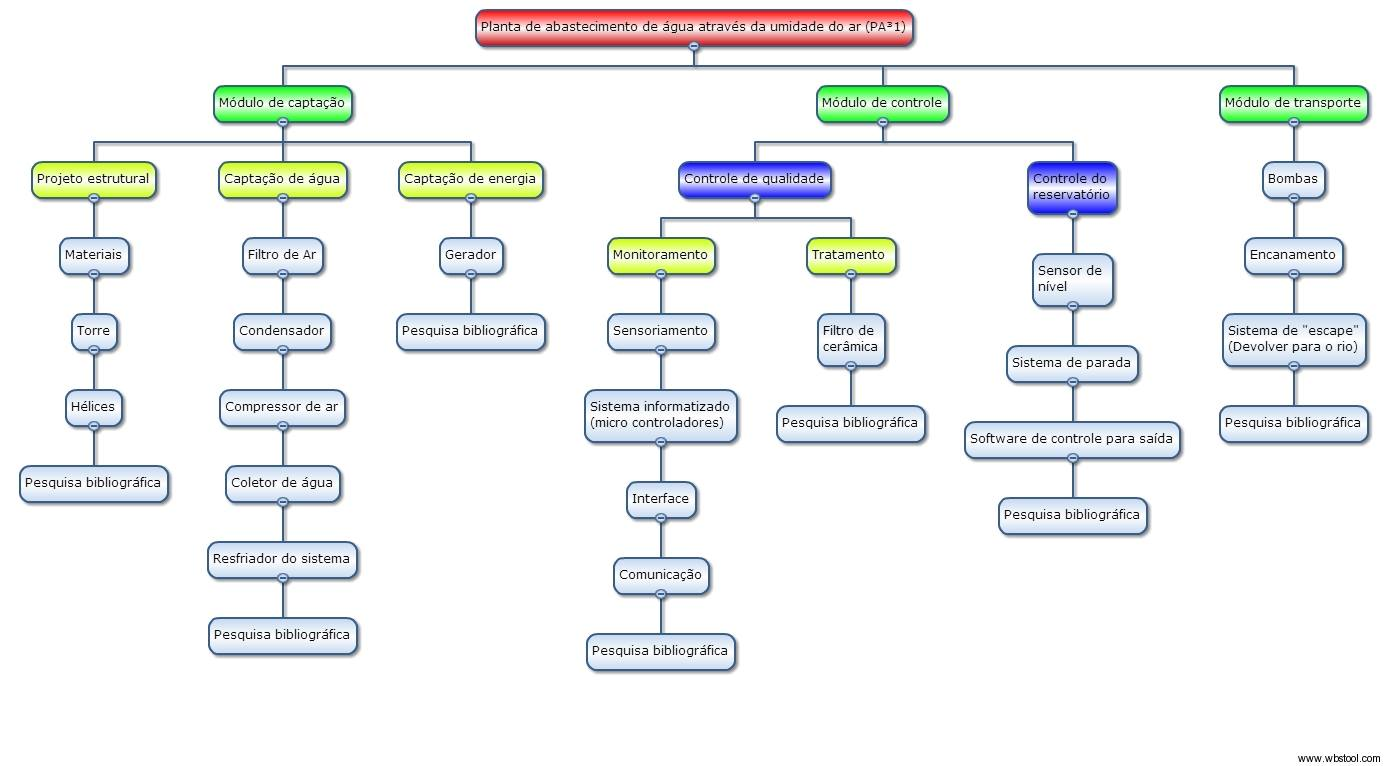
\includegraphics[scale=0.3]{editaveis/figuras/EAP}
\end{figure}
\FloatBarrier

\item Cronograma de marcos do projeto
O cronograma está descrito no item 5.3 da introdução.

\item Orçamento do projeto\\
Não há orçamento concreto para esse projeto em questão

\end{enumerate}
\section*{Metodologia}
A metodologia de desenvolvimento adotada neste projeto é uma adaptação de metodologias gerais de desenvolvimento
de produtos e serviços. Para a construção deste modelo de desenvolvimento foram selecionadas algumas técnicas de
projeto de produtos e serviços expostos em algumas obras de Slack (\citeyear{slack99}), Krajewski (\citeyear{krajewski96}) e Ramaswamy (\citeyear{ramaswamy96}).
Tais trabalhos descrevem formas de estabelecer etapas bem definidas para o desenvolvimento do projeto.\\
Como estrutura básica do projeto será adotada a seguinte metodologia, dividida em seis etapas:
\begin{figure}[h]
\centering
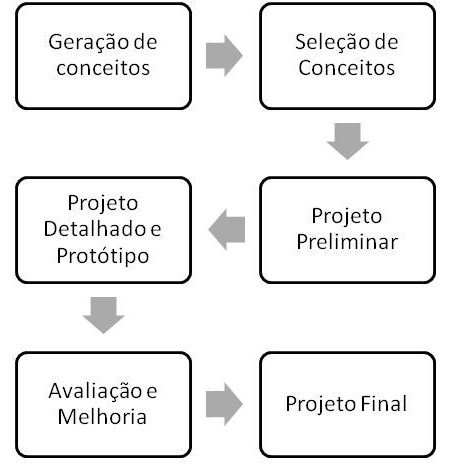
\includegraphics[scale=0.5]{editaveis/figuras/metodologia_de_desenvolvimento}
\end{figure}

\section*{Gestão de configuração}
A gestão de configuração foi o monitoramento das mudanças necessárias e viáveis para o progresso do projeto. As mudanças eram previamente colocadas em pauta na reunião e analisadas por todos, com o auxilio de dados e documentos sobre o porquê da mudança, depois de analisadas ela é aplicada e analisada novamente se a mesma não está em choque com as outras mudanças que  irão ser implementadas no mesmo momento.

\section*{Frequência de avaliação dos processos de gerenciamento do projeto}

Os processos de gerenciamento do projeto serão avaliados, primariamente, mensalmente, ou antes,
se surgirem problemas ou empecilhos para a continuação do projeto.

\section*{Alocação financeira para o gerenciamento do projeto.}

Não há dados de alocação financeira para o Gerenciamento de Projeto

\section*{Administração do plano de gerenciamento do projeto}
\begin{enumerate}
\item Responsável pelo plano:
\begin{itemize}
\item Rafael Abreu de Carvalho
\item Lais Rocha Carvalho
\end{itemize}
\item Frequência de atualização do plano de gerenciamento do projeto\\
	Terá no mínimo 1 atualização, o qual é a revisão programada ao termino desse plano. Poderá haver mais atualizações em menores escalas.

\end{enumerate}

\section*{Outros assuntos relacionados ao gerenciamento do projeto não previstos nesse plano}
Não há assuntos extras pertinentes ao plano de gerenciamento de Projeto

\section*{Documentos e planos auxiliares (anexos)}
\begin{itemize}
\item Plano de Gerenciamento das Comunicações
\item Plano de Gerenciamento de Escopo
\item Plano de Gerenciamento de Riscos
\item Plano de Gerenciamento de Recursos Humanos
\item Plano de Gerenciamento de Custos
\item Plano de Gerenciamento de Tempo
\item Plano de Gerenciamento de Qualidade
\item Plano de Gerenciamento das Aquisições
\item Cronograma do Projeto
\item EAP do projeto
\item Matriz de riscos do projeto


\end{itemize}

\section*{Documentos de referência}
\begin{itemize}
\item Declaração do Escopo Preliminar
\item Termo de abertura
\end{itemize}

\section*{Outras referências}
\begin{itemize}
\item PMBoK Guide 2004.
\end{itemize}

\section*{Assinaturas}
\begin{center}
Data: \rule{0.5cm}{0.1mm}/\rule{0.5cm}{0.1mm}/\rule{1cm}{0.1mm}     \\
\rule{13cm}{0.1mm}\\
ADRIANNY VIANA DE ARAÚJO AMORIM – GERENTE DE PROJETO\\

\end{center}
% \end{document}